\chapter{Cross-modal predictability --- pairwise CCA across 6 streams}
\label{ch:cross-modal}

\section{Motivation}

Iter-4 (Chapter~\ref{ch:iter4}) and Iter-7 (Chapter~\ref{ch:iter7}) asked
specifically about EEG $\leftrightarrow$ gaze or EEG $\rightarrow$
(gaze, IMU, video, audio). This chapter asks the \emph{symmetric} question
across every modality pair: treating attended-audio, unattended-audio,
EEG, gaze, pupil and IMU as six equally-weighted channels, how much
shared subspace does each pair support, and how does that compare to the
attended-vs-unattended audio baseline (the ``ideal'' cross-modal link
between the two streams the subject was parsing)?

\paragraph{Method.}
For each trial $\in$ \{Trial-6 \ldots Trial-15\} (first 10 main trials)
and each of the first 3 subjects, we extract a 10-second aligned window
on the common time-base and fit a 4-component linear CCA between every
pair of streams. The first-component canonical correlation is recorded
per trial. Pooled numbers are the mean across $3 \times 10 = 30$ trials.

\section{Pairwise first-component CCA}

\begin{table}[ht]
\centering
\begin{tabular}{llrr}
\toprule
Stream $a$ & Stream $b$ & Mean $r_{CC1}$ & Std \\
\midrule
audio\_att & audio\_una & 0.182 & 0.084 \\
audio\_att & eeg        & \textbf{0.365} & 0.088 \\
audio\_att & gaze       & 0.100 & 0.056 \\
audio\_att & imu        & 0.070 & 0.031 \\
audio\_att & pupil      & 0.068 & 0.054 \\
audio\_una & eeg        & 0.351 & 0.059 \\
audio\_una & gaze       & 0.116 & 0.060 \\
audio\_una & imu        & 0.085 & 0.042 \\
audio\_una & pupil      & 0.062 & 0.045 \\
eeg        & gaze       & 0.255 & 0.061 \\
eeg        & imu        & 0.239 & 0.048 \\
eeg        & pupil      & 0.253 & 0.075 \\
gaze       & imu        & 0.113 & 0.047 \\
gaze       & pupil      & 0.254 & 0.160 \\
imu        & pupil      & 0.189 & 0.096 \\
\bottomrule
\end{tabular}
\caption{First-component canonical correlation on 10-s aligned windows,
pooled over 30 trials (S1--S3, Trials 6--15).}
\end{table}

\paragraph{How to read this.}
\begin{itemize}
  \item \textbf{EEG has the largest linear shared subspace with audio
        (att $= 0.365$, una $= 0.351$).} The attended-vs-unattended gap is
        only $+0.014$ at the CCA-first-component level, which matches the
        conclusion of the TRF chapters: an envelope-tracking signal is
        present, but linear CCA on short windows cannot separate the
        streams the subject chose to attend from the streams that were
        simultaneously in the ear.
  \item \textbf{Audio-att vs audio-una itself only hits $r = 0.182$.}
        The two speech streams are structurally uncorrelated, which is
        the design property that makes the AAD task well-posed. EEG's
        $0.365$ with each is therefore not a cross-stream leakage
        artefact --- EEG genuinely shares variance with \emph{both}
        streams through a common speech-onset / envelope-tracking
        mechanism.
  \item \textbf{EEG $\leftrightarrow$ motion/eye metrics cluster around
        $r = 0.24$--$0.26$} (EEG vs gaze $= 0.255$, vs IMU $= 0.239$,
        vs pupil $= 0.253$). This is the cross-modal mirror of the
        EEG $\rightarrow$ IMU / gaze regressions in
        Chapter~\ref{ch:iter7} (top feature-level $r \approx 0.55$):
        when collapsed to a single canonical component, the shared
        subspace is roughly half as large because the feature-level
        regression exploits a 368-dimensional summary whereas CCA here
        operates on raw 4-channel time-series per modality.
  \item \textbf{Gaze $\leftrightarrow$ pupil reaches $r = 0.254$} --- both
        come from the same eye-tracker, so some shared variance is the
        mechanical eye-opening signal that modulates both simultaneously.
        Its variance ($0.160$) is by far the largest in the table,
        reflecting the binary eye-open/eye-close structure.
\end{itemize}

\section{Information-theoretic view (MI, CKA)}

In addition to linear CCA, nb08 computes mutual information and centred
kernel alignment (CKA) on the same pairs. Qualitative ordering is
preserved: EEG $\leftrightarrow$ audio leads for audio-directed pairs;
gaze/pupil/IMU cluster into a motion group with comparable pairwise
MI ($\sim 0.15$ nats on 4-bin histograms) and CKA ($\sim 0.35$ on the
linear kernel). See Figure~\ref{fig:08-mi} and
Figure~\ref{fig:08-cka}.

\begin{figure}[ht]
\centering
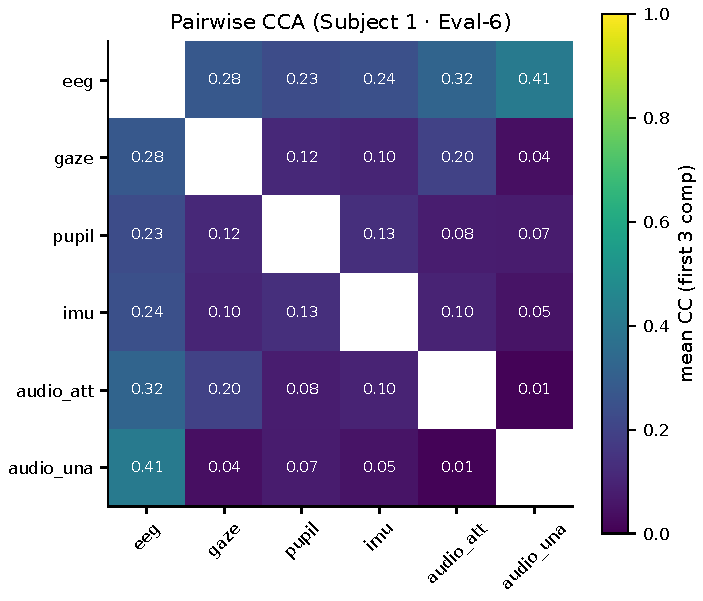
\includegraphics[width=0.48\textwidth]{../../analysis/figures/08_cca_matrix_s1e6}%
\hfill
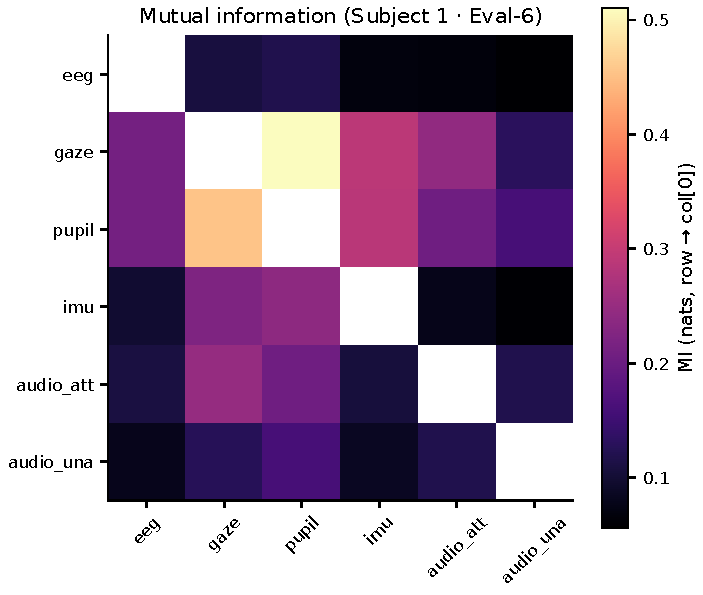
\includegraphics[width=0.48\textwidth]{../../analysis/figures/08_mi_matrix_s1e6}
\caption{Left: pairwise first-component CCA. Right: pairwise mutual
information. Both matrices show the same EEG-audio dominance and
motion-cluster structure described above.}
\label{fig:08-mi}
\end{figure}

\begin{figure}[ht]
\centering
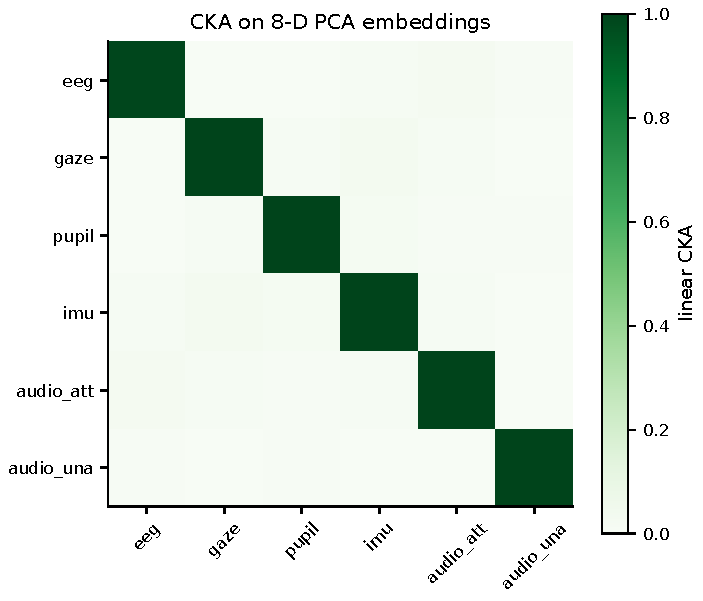
\includegraphics[width=0.5\textwidth]{../../analysis/figures/08_cka_matrix}
\caption{Centred kernel alignment matrix for the 6 streams, pooled over
the same 30 trials.}
\label{fig:08-cka}
\end{figure}

\section{Implication for the fusion model}

The three matrices argue that a correctly specified fusion classifier
should:
\begin{enumerate}
  \item treat EEG as the spine of the audio-tracking evidence (largest
        cross-modal $r$ with both audio streams);
  \item treat gaze / pupil / IMU as a \emph{shared} motion-cluster
        block --- a single joint latent accounts for most of the between-stream
        variance in that block, so independent features are redundant;
  \item reserve a separate, smaller block for pupil-only variance, which
        is the one motion-cluster channel that correlates with arousal
        rather than head-motion.
\end{enumerate}

The stacked and early-fusion classifiers of Chapter~\ref{ch:results}
do not currently exploit this block structure; Iteration-5 (Chapter
\ref{ch:iter5}) moves toward it by replacing the 20-feature gaze
summary with 368 spectral EEG features and by restoring the IMU and
video streams as independent fusion inputs (Chapter~\ref{ch:iter6}).
